%\documentclass[sigconf, authordraft]{acmart}
\documentclass[sigconf]{acmart}

\usepackage{algorithm}
\usepackage{algpseudocode}
\usepackage{amsmath}
\usepackage{amssymb}
\usepackage{mathtools}

\usepackage{booktabs} % For formal tables
\usepackage[outdir=./]{epstopdf}
\usepackage{graphicx}
\usepackage{listings}
\usepackage{setspace}
%\doublespacing
\lstset{
  language=C++,
  basicstyle=\ttfamily\footnotesize,
  showspaces=false,
  showtabs=false,
  tabsize=2,
  frame=single,
}
% Copyright
%\setcopyright{none}
%\setcopyright{acmcopyright}
%\setcopyright{acmlicensed}
\setcopyright{rightsretained}
%\setcopyright{usgov}
%\setcopyright{usgovmixed}
%\setcopyright{cagov}
%\setcopyright{cagovmixed}


% DOI
\acmDOI{10.1145/nnnnnnn.nnnnnnn}

% ISBN
\acmISBN{978-x-xxxx-xxxx-x/YY/MM}

% Conference
\acmConference[GECCO '19]{the Genetic and Evolutionary Computation Conference 2019}{July 13--17, 2019}{Prague, Czech Republic}
\acmYear{2019}
\copyrightyear{2019}

%\acmArticle{4}
\acmPrice{15.00}

% These commands are optional
%\acmBooktitle{Transactions of the ACM Woodstock conference}
%\editor{Jennifer B. Sartor}
%\editor{Theo D'Hondt}
%\editor{Wolfgang De Meuter}


\begin{document}
%\title{Cache-Aware Parallel Particle Swarm Optimization}
\title{Two Simple Tricks for Cache-Aware, Parallel Particle Swarm Optimization}
%%% The submitted version for review should be ANONYMOUS
\author{Jeff Hajewski}
\orcid{1234-5678-9012}
\affiliation{%
  \institution{University of Iowa\\ Department of Computer Science}
  \city{Iowa City} 
  \state{Iowa} 
  \postcode{52242}
}
\email{jeffrey-hajewski@uiowa.edu}

\author{Suely Oliveira}
\affiliation{%
  \institution{University of Iowa\\ Department of Computer Science}
  \city{Iowa City}
  \state{Iowa} 
  \postcode{52242}
}
\email{suely-oliveira@uiowa.edu}

% The default list of authors is too long for headers.
\renewcommand{\shortauthors}{J. Hajewski et al.}


\begin{abstract}
  In this work we present a general framework for building cache-efficient,
  parallel Particle Swarm Optimization implementations.  While prior work
  \cite{cache-pso} has explored cache-efficient designs for PSO in the
  sequential setting, we show that this work does not naively generalize to the
  parallel setting.  Specifically, we show that spreading blocks of work across
  threads maintains data-locality and breaking the algorithm into as many
  functional components as possible allows the compiler to more effectively
  optimize each functional unit.  In our experiements using GCC 8.1
  we found auto-vectorized code from the compiler was as efficient, and
  sometimes more efficient, than our hand-rolled functions using AVX2
  instructions.  Our implementation out performs the standard object-oriented
  implementation of PSO by margins has great as 50\% in both the parallel and
  sequential settings. Further, we beat the naively parallelized,
  cache-efficient algorithm by more than 10-20\% in a number of settings.
\end{abstract}

%
% The code below should be generated by the tool at
% http://dl.acm.org/ccs.cfm
% Please copy and paste the code instead of the example below. 
%
\begin{CCSXML}
<ccs2012>
<concept>
<concept_id>10010147.10010169.10010170.10010171</concept_id>
<concept_desc>Computing methodologies~Shared memory algorithms</concept_desc>
<concept_significance>500</concept_significance>
</concept>
<concept>
<concept_id>10010147.10010178</concept_id>
<concept_desc>Computing methodologies~Artificial intelligence</concept_desc>
<concept_significance>500</concept_significance>
</concept>
<concept>
<concept_id>10010147.10010341.10010349.10010355</concept_id>
<concept_desc>Computing methodologies~Agent / discrete models</concept_desc>
<concept_significance>300</concept_significance>
</concept>
</ccs2012>
\end{CCSXML}

\ccsdesc[500]{Computing methodologies~Shared memory algorithms}
\ccsdesc[500]{Computing methodologies~Artificial intelligence}
\ccsdesc[300]{Computing methodologies~Agent / discrete models}

\keywords{Particle Swarm Optimization, cache-aware algorithms, artificial intelligence}


\maketitle

\section{Introduction}
Particle Swarm Optimization (PSO) \cite{pso} is an optimization technique commonly used for
finding the global optimum of a nonlinear function. PSO work by emulating swarms
that occur in nature (e.g., a flock of birds) such that each particle searches
locally in the direction of its best seen position as well as the best seen
position of the swarm. The swarm maintains a global best position (the position
with the optimal fitness value) and the goal is for this global best position to
quickly converge to the global minimum (maximum) of the nonlinear function being
optimized.  The challenge comes in the form of required compute power -- due to
the curse of dimensionality, a high-dimensional problem requires a large number
of particles. Efficient algorithm design coupled with efficient implementation
is essential for handling large simulations of particles. In the authors'
personal experience, making a heap allocation in the wrong spot or even
something as simple as generating a random number in the wrong location can
increase the runtime of a simulation $1000\times$.\\
The contributions of this work are:
\begin{enumerate}
\item An improved cache-efficient algorithm for parallel PSO
\item A general framework for writing efficient PSO implementations
\end{enumerate}

While there is a large body of work on parallel PSO using various threading
techniques or even GPGPU programming, the goal of our work is to provide a set
of techniques, tools, and modifications to the standard cache-efficient PSO
algorithm that are simple to understand and use. The average user of a PSO
algorithm likely does not have the specialized knowledge to write an efficient
CUDA implementation or to implement efficient management and coordination of
threads. Rather than provide a highly specialized implementation, we focus on
simplicity. For parallelism, we utilize OpenMP. We also demonstrate that while
custom written vectorized code can often be hard to beat, utilizing
auto-vectorization through the compiler along with well designed code can be
nearly as effective without requiring specialized knowledge or low-level
programming.

The organization of the paper is as follows. In section \ref{sec:pso} we give a
breif overview of PSO, followed by an overview of cache-aware algorithms and the
challenges encountered in parallel algorithms in secion \ref{sec:cache}. We
present our updated PSO algorithm and implementation guidelines in section
\ref{sec:algo} followed by experimental results in section \ref{sec:results}.

\section{Particle Swarm Optimization}\label{sec:pso}
Particle Swarm Optimization can be simplified into the update of two formulas:
one for a particle's velocity and the other for the particle's position. Define
$\textbf{pbest}$ as the position corresponding to the best seen fitness value
for a given particle (i.e., the local best), $\textbf{gbest}$ as the position
corresponding to the the best seen fitness value globally, and $\textbf{p}$ as
the current position of the given particle. The update formula for velocity is
given by equation (\ref{eq:velocity} and Table \ref{tab:constants} describes
the interpretation of the constants.

\begin{multline}\label{eq:velocity}
  v_i(t+1) = \omega v_i (t) + c_1 r_1 (\textbf{pbest}_i(t) - \textbf{p}_i(t)) \\
  + c_2 r_2 (\textbf{gbest}_i(t) - \textbf{p}_i(t))
\end{multline}

Once the velocity is computed, the position update is given by equation
(\ref{eq:position}).

\begin{equation}\label{eq:position}
  \textbf{p}_i(t+1) = \textbf{p}_i(t) + \textbf{v}_i(t)
\end{equation}

\begin{table}
  \caption{Description of the velocity update constants.}\label{tab:constants}
  \begin{tabular}{ll}\toprule
  \textbf{Constant} & \textbf{Description}\\\midrule
  $\omega$ & Momentum\\
  $c_1$ & Explore towards local best\\
  $c_2$ & Exploration towards global best\\
  $r_1$ and $r_2$ & sampled from $U(0,1)$\\\bottomrule
  \end{tabular}
\end{table}

Algorithm \ref{alg:pso} describes the basic PSO algorithm.

\begin{algorithm}
  \caption{Basic PSO algorithm.}\label{alg:pso}
  \begin{algorithmic}[1]
    \Procedure{PSO}{N}
    \State $\texttt{particles} \gets \texttt{initialize}(N)$
    \Repeat
    \For{$\textbf{p} \in \texttt{particles}$}
    \State \texttt{p.UpdateVelocity(\textbf{gbest})}
    \State \texttt{p.UpdatePosition()}
    \EndFor
    \Until Convergence
    \EndProcedure
  \end{algorithmic}
\end{algorithm}

Particles are initialized randomly within the bounds of the search space
$[\texttt{x\_min}, \texttt{x\_max}]$. Some implementations also set a random
intiail velocity for each particle; however, we found it simpler and equally
effective to initialize all particles with zero velocity. When a particle
reaches the boundary of the search space, we reflect it off the boundary back
into the search space by making the resepctive velocity component the negation
of its prior value and setting the particle position to the boundary value.

Our implementation allows for a predefined minimum and maximum value for
components of the velocity vector -- in practice these should be no greater than
the diameter of the search space.

\section{Cache-aware Design}\label{sec:cache}
Modern \texttt{x86\_64} CPUs typically have three tiers of cache: L1, L2, and
L3. L1 cache is the fastest but has the smallest amount of storage. The caches
decrease in speed and increase in storage as one descends the cache
hierarchy. When data is loaded into a register the first step is to check the
cache, then RAM, and lastly disk. Rather than load a single piece of data from
RAM into cache, CPUs load a cache line, which is typically 64B. A standard cache
line corresponds to 16 32-bit numbers or 8 64-bit numbers. A cache-aware
algorithm utilizes this information by grouping data such that data utilized by
the algorithm in temporal proximity is physically stored spatially close. This
is referred to as data locality. In other words, we want to keep data that is
accessed at around the same time as close together as possible. This reduces
access to RAM and in the worst case, disk, both of which are substantially more
costly than accessing cache.

\subsection{Data-Oriented Design}
We can use the idea of data locality and cache-aware algorithm design to
influence the design of our programs. This is known as data-oriented design and
is a very common technique in the video game industry where writing highly
efficient and performant code is a fundamental requirement. Data-oriented design
differs from object-oriented design in that data is grouped based on access
paterns rather than logical patterns. Figure \ref{fig:particle} shows a typical
object-oriented design of a particle class.

\begin{figure}
  \lstinputlisting{../code/particle.cpp}
  \caption{Example of a Particle class using object-oriented
    design.}\label{fig:particle}
\end{figure}

The standard object-oriented implementation of PSO would be to store the
particles in a vector, where each entry of the vector is the particle object of
a specific particle. When a particle gets loaded into cache from memory the
cache line will contain three \texttt{T*} pointers, the three constant values
$c_1$, $c_2$, and $\omega$, and two function pointers to the fitness and and
velocity update functions. The fitness function does not change from particle to
particle, so at a minimum this presents us with an opportunity for
optimizing our implementation.

Figure \ref{fig:particles} shows an example of a data-oriented design
approach. The key aspects with this design is that particle positions are stored
in a vector, particle velocities are stored in a vector, and particle best
positions are stored in a vector. Rather than encapsulate particle specific
information in a particle object, we place that information in a vector along
with similar information of other particles. The advantage is data
locality. When we update the velocity of one particle, we will be updating the
velocity of other particles. For example, loading the first velocity vector (we
can think of this is a \texttt{T*} pointer for simplicity), the next seven
velocity pointers will also be pulled into cache because they are on the same
cache line. Compare this with the object-oriented approach where we would need
seven different loads from main memory to get these pointers since each particle
object took up an entire cache line.
\begin{figure}
  \lstinputlisting{../code/particles.cpp}
  \caption{Example of a data-oriented design modeling all particles in a PSO
    simulation.}\label{fig:particles}
\end{figure}

\begin{algorithm}
  \caption{Cache-aware algorithm for PSO.}\label{alg:pso-cache}
  \begin{algorithmic}[1]
    \Procedure{PSO-DO}{N}
    \State $\texttt{vel} \gets \texttt{initialize}(N)$ \Comment{velocity vectors}
    \State $\texttt{pos} \gets \texttt{initialize}(N)$ \Comment{position vectors}
    \State $\texttt{bpos} \gets \texttt{pos}$ \Comment{best position vectors}

    \Repeat
    \State $\texttt{gbest} = \text{argmin}_{\texttt{pos}}\texttt{fitness}(p)$
    \For{$(i, v) \in \texttt{enumerate}(\texttt{vel})$}
    \State $\texttt{local} \gets (\texttt{pos}[i] -
    \texttt{bpos}[i])$
    \State $\texttt{global} \gets  (\texttt{pos}[i]
    - \texttt{gbest})$
    \State $v \gets \omega v + c_1 r_1 \texttt{local}  + c_2 r_2 \texttt{global}$
    \EndFor
    \For{$(p, v) \in \texttt{zip}(\texttt{pos}, \texttt{vel})$}
    \State p += v
    \EndFor
    \Until convergence
    \EndProcedure
  \end{algorithmic}
\end{algorithm}

\section{Cache-aware, Parallel PSO}\label{sec:algo}
We make several improvements to the framework for cache-efficient PSO proposed
in \cite{cache-pso}. While none of these improvements is a major structural
change to the algorithm of PSO or the data-oriented design, we found that the
net effect was a dramatic improvement in performance.

\paragraph{Random Weights} One of the major speed-ups we achieved was through
the placement of the random weights $r_1$ and $r_2$. The generation of these
values vary throughout the literature. We found using the same random values for
every component of the velocity vector and sampilng new values each time the
velocity vector is encountered provided the best trade-off. Sampling too often
is expensive while sampling too infrequently slows convergence due to a lack of
diversity in search directions.

\paragraph{Auto-vectorization}
The difference between Figure \ref{fig:naive-par} and Figure
\ref{fig:efficient-par} is pulling the inner loop into a separate function. This
allows the compiler to more easily optimize that piece of code by making the
relationship between the different vectors clear -- there is no pointer aliasing
between \texttt{i} values. In our experiments, for simple loops like this it is
difficult to beat the compiler by hand-writing AVX instructions, especially
without domain expertise in writing efficient, low-level code.

\begin{algorithm}
  \caption{Cache-aware parallel PSO}\label{alg:par-pso}
  \begin{algorithmic}[1]
    \Procedure{Parallel-PSO}{N}
    \State $\texttt{n\_threads} \gets \texttt{getn\_hardware\_threads}()$
    \State $\texttt{tp} \gets \texttt{ThreadPool}()$
    \State $\texttt{vel} \gets \texttt{initialize}(N)$
    \State $\texttt{pos} \gets \texttt{initialize}(N)$
    \State $\texttt{bpos} \gets \texttt{pos}$

    \State $n = N/\texttt{n\_threads}$ \Comment{Assume $N \mod
      \texttt{n\_threads} = 0$}
    \For{$(i, t) \in \texttt{enumerate}(\texttt{tp})$}
    \State $vs \gets \texttt{vel}[ni:n(i+1)]$
    \State $ps \gets \texttt{pos}[ni:n(i+1)]$
    \State $bps \gets \texttt{bpos}[ni:n(i+1)]$
    \State $\texttt{t(Run}(vs, ps, bps))$
    \EndFor
    \For{$t \in \texttt{tp}$}
    \State \texttt{t.join()}
    \EndFor
    \EndProcedure
  \end{algorithmic}
  \begin{algorithmic}[1]
    \Procedure{Run}{\texttt{vs}, \texttt{ps}, \texttt{bps}}
    \State $n \gets \texttt{ps.size()}$
    \Repeat
    \For{$i = 1 \to n$}
    \State $\texttt{gbest} \gets \min\{\texttt{gbest}, \texttt{po}$
    \EndFor
    \For{$i = 1 \to n$}
    \State 
    \EndFor
    \Until convergence
    \EndProcedure
  \end{algorithmic}
\end{algorithm}

\begin{figure}
  \lstinputlisting{../code/naive_par.cpp}
  \caption{Naive loop parallelization with OpenMP.}\label{fig:naive-par}
\end{figure}

\begin{figure}
  \lstinputlisting{../code/efficient_par.cpp}
  \caption{Efficient loop parallelization with OpenMP.}\label{fig:efficient-par}
\end{figure}

\section{Results}\label{sec:results}
We test our algorithm on both the Rastrigin \cite{rastrigin} and Ackley \cite{ackley} functions
in high dimensions. The three-dimensional plots of these functions are given in Figures
\ref{fig:rastrigin} and \ref{fig:ackley}, respectively.  The goals fo the
experiments are:
\begin{enumerate}
  \item Investigate the relationship between dimension and number of particles
    with respect to performance of the cache-aware parallel implementation to
    the object-oriented parallel implementation
\end{enumerate}

\begin{figure}
  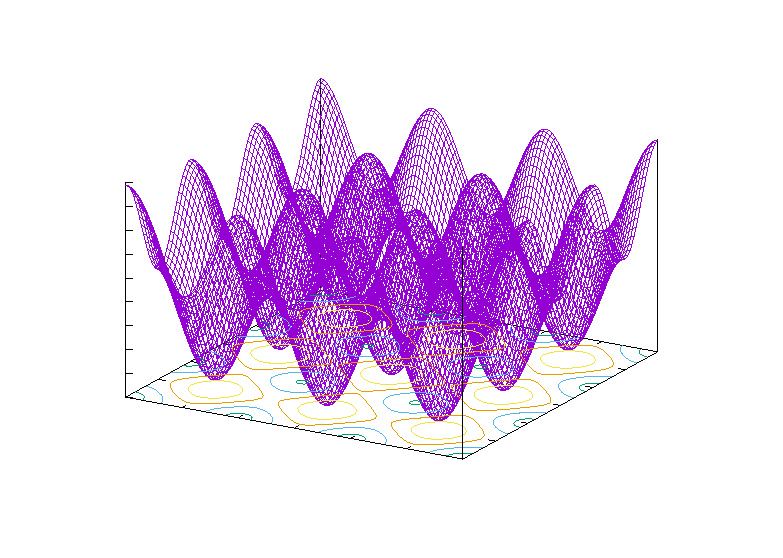
\includegraphics[width=\columnwidth]{../img/output/rastrigin}
  \caption{The Rastrigin function in three dimensions.}\label{fig:rastrigin}
\end{figure}

\begin{figure}
  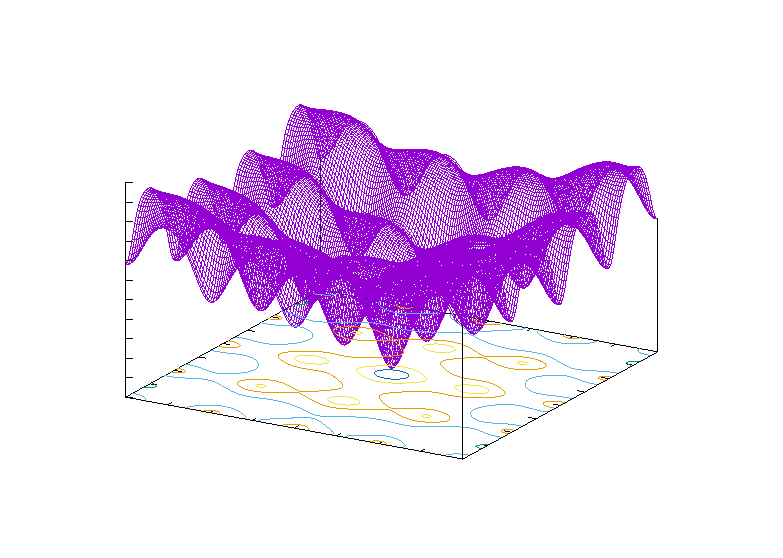
\includegraphics[width=\columnwidth]{../img/output/ackley}
  \caption{The Ackley function in three dimensions.}\label{fig:ackley}
\end{figure}


\section{Conclusion}
This paragraph will end the body of this sample document.
Remember that you might still have Acknowledgments or
Appendices; brief samples of these
follow.  There is still the Bibliography to deal with; and
we will make a disclaimer about that here: with the exception
of the reference to the \LaTeX\ book, the citations in
this paper are to articles which have nothing to
do with the present subject and are used as
examples only.
%\end{document}  % This is where a 'short' article might terminate




\bibliographystyle{ACM-Reference-Format}
\bibliography{bibliography.bib} 

\end{document}
